\documentclass[solutionorbox,answers]{exam}
% \documentclass[solutionorbox]{exam}

%%%%%%%%%%%%%%%%%%%%%%%%%%%%%%%%%%%%%%%%%%%%%%%%%%%%%%%%%%%%%%%
% Update to change header
\newcommand{\courseName}{CS 577}
\newcommand{\assignmentName}{Assignment 1 -- Discrete Review}
\newcommand{\semester}{Spring 2023}
%%%%%%%%%%%%%%%%%%%%%%%%%%%%%%%%%%%%%%%%%%%%%%%%%%%%%%%%%%%%%%%

\usepackage[utf8]{inputenc}
\usepackage[T1]{fontenc}

\usepackage{amsmath}
\usepackage{amsfonts}
\usepackage{amsthm}
\usepackage{booktabs}
\usepackage{tkz-graph}
\usepackage[ruled]{algorithm2e}
\usepackage{graphicx}
\usepackage{multicol}

\usepackage{listings}
\lstset{basicstyle=\ttfamily,
  showstringspaces=false,
  commentstyle=\color{red},
  keywordstyle=\color{blue}
}

\usepackage{hyperref}

\pagestyle{headandfoot}
\runningheadrule
\firstpageheader{\courseName}{\huge \assignmentName}{\semester}
\runningheader{\courseName}
{\assignmentName}
{\semester}
\firstpagefooter{}{}{}
\runningfooter{}{Page \thepage\ of \numpages}{}

\begin{document}

\begin{center}
\fbox{\parbox{5.5in}{\centering
Answer the questions in the boxes provided on the
question sheets. If you run out of room for an answer,
add a page to the end of the document. \\
\vspace{0.1in}
Related Readings: \url{http://pages.cs.wisc.edu/~hasti/cs240/readings/}
}}
\end{center}
\vspace{0.1in}
\makebox[0.48\textwidth]{Name:\enspace\hrulefill} \qquad
\makebox[0.48\textwidth]{Wisc id:\enspace\hrulefill}

\begin{questions}

\section*{Logic}

  \question
  Using a truth table, show the equivalence of the following statements.
\begin{parts}
  \part
  $P \vee (\neg P \wedge Q) \equiv P \vee Q$
  \nopagebreak
  \begin{solutionbox}{2in}\\
    
  \end{solutionbox}
  
  \part
  $\neg P \vee \neg Q \equiv \neg (P \wedge Q)$
  \nopagebreak
  \begin{solutionbox}{2in}\\
    
  \end{solutionbox}
  
  \part
  $\neg P \vee P \equiv \text{true}$
  \nopagebreak
  \begin{solutionbox}{2in} \vspace{1em} \\

  \end{solutionbox}
  
  \part
  $P \vee (Q \wedge R) \equiv (P \vee Q) \wedge (P \vee R)$
  \nopagebreak
  \begin{solutionbox}{3in}\\
   
  \end{solutionbox}
  
\end{parts}

\newpage
\section*{Sets}


  \question
  Based on the definitions of the sets $A$ and $B$, calculate the following: $|A|$, $|B|$, $A \cup B$, $A \cap B$, $A \setminus B$, $B \setminus A$.

  \begin{parts}
    \part
    $A = \{1, 2, 6, 10\}$ and $B = \{2, 4, 9, 10\}$
    \nopagebreak
    \begin{solutionbox}{2in}
      
    \end{solutionbox}
    \part
    $A = \{x \mid x \in \mathbb{N}\}$ and $B = \{x \in \mathbb{N} \mid x \text{ is even} \}$
    \nopagebreak
    \begin{solutionbox}{2in}
      
    \end{solutionbox}

  \end{parts}

\section*{Relations and Functions}

\question
For each of the following relations, indicate if it is reflexive, antireflexive, symmetric, antisymmetric, or transitive.

\begin{parts}
\part
$\{(x,y) : x \le y\}$
\begin{solutionbox}{0.5in}

\end{solutionbox}
\part
$\{(x,y) : x > y\}$
\begin{solutionbox}{0.5in}

\end{solutionbox}
\newpage
\part
$\{(x,y) : x < y\}$
\begin{solutionbox}{0.5in}

\end{solutionbox}
\part
$\{(x,y) : x = y\}$ 
\begin{solutionbox}{0.5in}

\end{solutionbox}
\end{parts}

\question
For each of the following functions (assume that they are all $f: \mathbb{Z} \to \mathbb{Z}$), indicate if it is surjective (onto), injective (one-to-one), or bijective.

\begin{parts}
\part
$f(x) = x$
\begin{solutionbox}{0.5in}

\end{solutionbox}
\part
$f(x) = 2x - 3$
\begin{solutionbox}{0.5in}

\end{solutionbox}
\part
$f(x) = x^2$
\begin{solutionbox}{0.5in}

\end{solutionbox}
\end{parts}
\question
Show that $h(x) = g(f(x))$ is a bijection if $g(x)$ and $f(x)$ are bijections.

\begin{solutionbox}{3in}

\end{solutionbox}

\section*{Induction}
\label{sec:induction}

\question
Prove the following by induction.

\begin{parts}
  \part
  $\sum_{i = 1}^n i = n(n+1)/2$
  \begin{solutionbox}{2.3in}\\

  \end{solutionbox}
  
  \part
  $\sum_{i = 1}^n i^2 = n(n+1)(2n+1)/6$
  \begin{solutionbox}{2.3in}\\

  \end{solutionbox}
  
  \part
  $\sum_{i = 1}^n i^3 = n^2(n+1)^2/4$
    \begin{solutionbox}{2.3in}\\

  \end{solutionbox}
\end{parts}

\section*{Graphs and Trees}
\label{sec:graphs-trees}

\question 
Give the adjacency matrix, adjacency list, edge list, and incidence matrix for the following graph. \\
\begin{minipage}{0.3\linewidth}
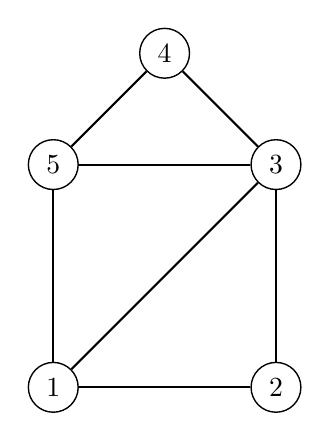
\begin{tikzpicture}
\GraphInit[vstyle=Normal]
\SetGraphUnit{2}
\begin{scope}[rotate=-135]
\Vertices{circle}{1,2,3,5}
\end{scope}
\NOEA[unit=1.414](5){4}
\Edges(1,2,3,5,4,3,1,5)
\end{tikzpicture}
\end{minipage}
\qquad
\begin{minipage}{0.6\linewidth}
\begin{solutionbox}{3.8in}\\

\end{solutionbox}
\end{minipage}
\question
How many edges are there is a complete graph of size $n$? Prove by induction.

\begin{solutionbox}{3.8in}

\end{solutionbox}

\question
Draw all possible (unlabelled) trees with 4 nodes.

\begin{solutionbox}{3.8in}
  
\end{solutionbox}

\question
Show by induction that, for all trees, $|E| = |V| - 1$.

\begin{solutionbox}{3.8in}

\end{solutionbox}

\section*{Counting}
\label{sec:counting}

\question
How many 3 digit pin codes are there?

\begin{solutionbox}{0.5in}

\end{solutionbox}

\question
What is the expression for the sum of the $i$th line (indexing starts at 1) of the following: \\
\begin{minipage}{0.1\textwidth}
\begin{align*}
 & 1        \\
 & 2\ 3      \\
 & 4\ 5\ 6    \\
 & 7\ 8\ 9\ 10 \\
 & \vdots
\end{align*}
\end{minipage}
\begin{minipage}{0.89\linewidth}
  \begin{solutionbox}{2in} \\
  
\end{solutionbox}
\end{minipage}

\question
A standard deck of 52 cards has 4 suits, and each suit has card number 1 (ace) to 10, a jack, a queen, and a king. A standard poker hand has 5 cards. For the following, how many ways can the described hand be drawn from a standard deck.

\begin{parts}
  \part
  A royal flush: all 5 cards have the same suit and are 10, jack, queen, king, ace.
  \begin{solutionbox}{0.5in}

  \end{solutionbox}

  \part
  A straight flush: all 5 cards have the same suit and are in sequence, but not a royal flush.
  \begin{solutionbox}{0.8in}

  \end{solutionbox}
  
  \part
  A flush: all 5 cards have the same suit, but not a royal or straight flush.
  \begin{solutionbox}{0.8in}

  \end{solutionbox}

  \part
  Only one pair (2 of the 5 cards have the same number/rank, while the remaining 3 cards all have different numbers/ranks):
  \begin{solutionbox}{0.8in}

  \end{solutionbox}
  
\end{parts}

\section*{Proofs}
\label{sec:proofs}

\question
Show that $2x$ is even for all $x \in \mathbb{N}$.

\begin{parts}
  \part
  By direct proof.
  \begin{solutionbox}{2in}

  \end{solutionbox}
  
  \part
  By contradiction.
    \begin{solutionbox}{2in}

    \end{solutionbox}
  \end{parts}

\question
For all $x,y \in \mathbb{R}$, show that $|x + y| \le |x| + |y|$. (Hint: use proof by cases.)
\begin{solutionbox}{3in}

\end{solutionbox}

\section*{Program Correctness (and Invariants)}
\label{sec:program-correctness}

\question
For the following algorithms, describe the loop invariant(s) and prove that they are sound and complete.
\begin{parts}
  \part 
  \begin{algorithm}[H]
    \DontPrintSemicolon
    \KwIn{$a$: A non-empty array of integers (indexed starting at 1)}
    \KwOut{The smallest element in the array}
    \Begin{
      $min \gets \infty$\;
      \For{$i \gets 1$ \KwTo len($a$)}{
        \If{$a[i] < min$} {
          $min \gets a[i]$\; 
        }
      }
      \Return{$min$}\;
    }
    \caption{findMin}
  \end{algorithm}
  \begin{solutionbox}{5.9in} 

  \end{solutionbox}

    \part 
  \begin{algorithm}[H]
    \DontPrintSemicolon
    \KwIn{$a$: A non-empty array of integers (indexed starting at 1)}
    \KwOut{$a$ sorted from largest to smallest}
    \SetKw{Break}{break}
    \Begin{
      \For{$i \gets 2$ \KwTo len($a$)}{
        $val \gets a[i]$\;
        \For{$j \gets 1$ \KwTo $i - 1$}{
          \If{$val > a[j]$} {
            shift $a[j..i-1]$ to $a[j+1..i]$\;
            $a[j] \gets val$\;
            \Break
          }
        }
      }
      \Return{$a$}\;
    }
    \caption{InsertionSort}
  \end{algorithm}
  \begin{solutionbox}{5.9in}
    
  \end{solutionbox}
  
\end{parts}
\section*{Recurrences}
\label{sec:recurrences}

\question
Solve the following recurrences.

\begin{parts}
  \part
  $c_0 = 1; c_{n} = c_{n-1} + 4$

  \begin{solutionbox}{3.7in}

  \end{solutionbox}

  \part
  $d_0 = 4; d_{n} = 3 \cdot d_{n-1} $

  \begin{solutionbox}{3.7in}

  \end{solutionbox}

  \part
  $T(1) = 1; T(n) = 2T(n/2) + n$ (An upper bound is sufficient.)

  \begin{solutionbox}{3.9in}

  \end{solutionbox}

  \part
  $f(1) = 1; f(n) = \sum_{1}^{n-1}\left(i \cdot f(i)\right)$\\ (Hint: compute $f(n+1)-f(n)$ for $n>1$)

  \begin{solutionbox}{3.9in}

  \end{solutionbox}

  
\end{parts}

\section*{Coding Question}

Most assignments will have a coding question. You can code in C, C++, C\#, Java, Python, or Rust. You will submit a Makefile and a source code file.
\vspace{-0.5cm}

\paragraph{Makefile:} In the Makefile, there needs to be a build command and a run command. Below is a sample Makefile for a C++ program. You will find this Makefile in assignment details. Download the sample Makefile and edit it for your chosen programming language and code.

\lstinputlisting[language=Make]{Makefile}

\paragraph{HelloWorld Program Details}

The input will start with a positive integer, giving the number of instances that follow. For each instance, there will be a string. For each string $s$, the program should output Hello, $s$! on its own line.

A sample input is the following:
\begin{verbatim}
3
World
Marc
Owen
\end{verbatim}

The output for the sample input should be the following:
\begin{verbatim}
Hello, World!
Hello, Marc!
Hello, Owen!
\end{verbatim}

\end{questions}

\end{document}
